\documentclass[11pt]{article}
\usepackage{graphicx}
\usepackage[margin=0.5in]{geometry}
\usepackage{float}
\graphicspath{ {./img/} }
\renewcommand{\figurename}{Fig.}
\begin{document}

\title{ Clasificaci\'on de flores usando el dataset Iris por medio de una red neuronal }
\author{Orlando Hernandez Nu\~nez. Juan Alejandro Bernal Gallego}
\date{05 de Noviembre del 2019}
\maketitle
\section{Introducci\'on}
En el presente trabajo se describe el proceso llevado a cabo para entrenar una red neuronal con el objetivo de clasificar una flor atendiendo a sus caracter\'isticas f\'isicas.
\section{Red neuronal}
\subsection{Descripci\'on del dataset}
El dataset con el que se realiza el entrenamiento de la red neuronal se compone de 100 registros o muestras,
cada uno de ellos con la medida de longitud y ancho de p\'etalos y s\'epalos adem\'as de su respectiva clasificaci\'on.
\begin{figure}[H]
    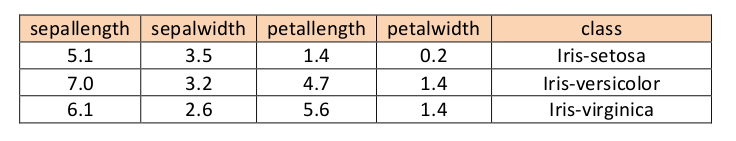
\includegraphics[width=13cm, height=7cm]{dt_example}
    \centering
    \caption{Estructura y registros del dataset}
    \label{fig:dt_example}
\end{figure}
\subsection{Arquitectura de la red neuronal}
La red neuronal posee tres capas, una capa de entrada donde se tomar\'an 4 valores, que corresponden a las caracter\'isticas físicas del tama\~no de una flor; una capa intermedia oculta la cual
posee 1 2 \'o 3 neuronas y finalmente, una capa de salida que esta compuesta de una neurona.
\begin{figure}[H]
    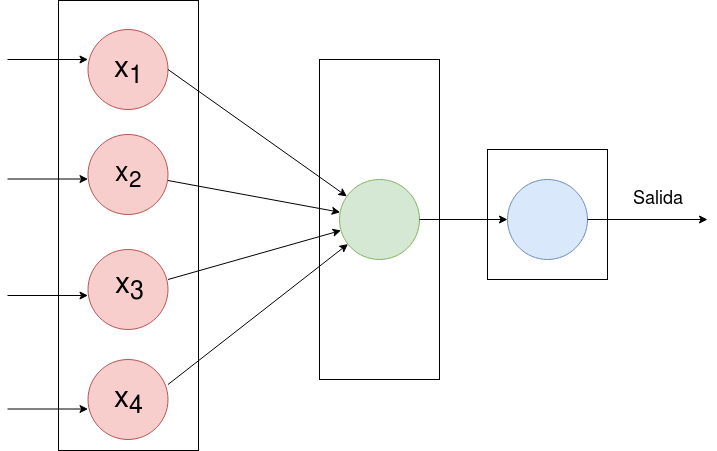
\includegraphics[width=10cm, height=8cm]{1hn}
    \centering
    \caption{Red neuronal con 1 neurona en la capa oculta}
    \label{fig:1hn}
\end{figure}

\begin{figure}[H]
    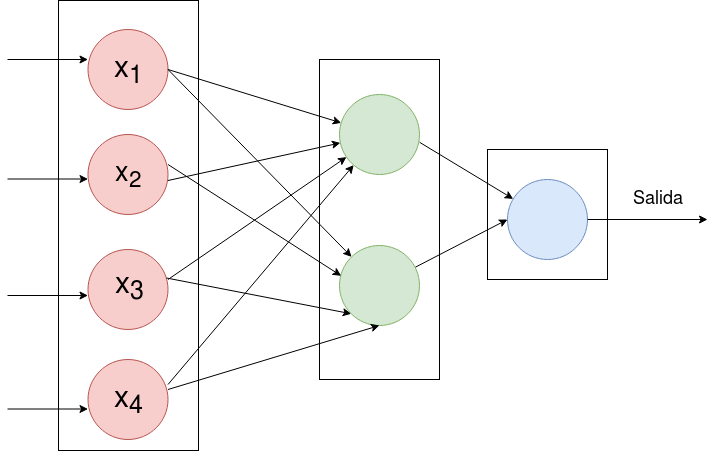
\includegraphics[width=10cm, height=8cm]{2hn}
    \centering
    \caption{Red neuronal con 2 neuronas en la capa oculta}
    \label{fig:2hn}
\end{figure}
\begin{figure}[H]
    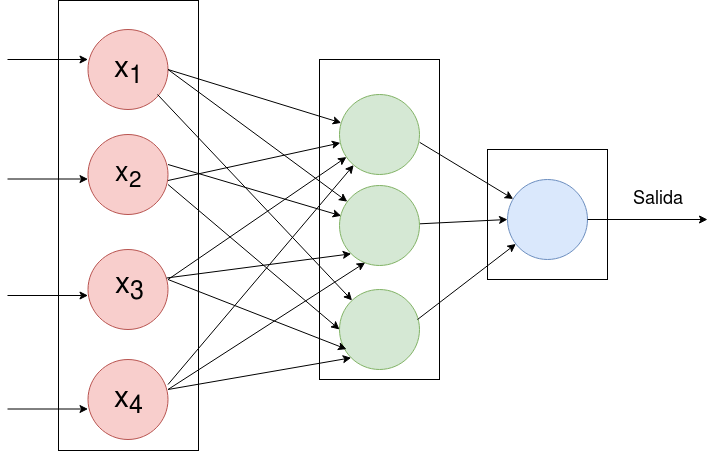
\includegraphics[width=10cm, height=8cm]{3hn}
    \centering
    \caption{Red neuronal con 3 neuronas en la capa oculta}
    \label{fig:3hn}
\end{figure}
\subsection{Entrenamiento}
De manera aleatoria se escoge  el 80\% del dataset para entrenar la red neuronal y el porcentaje
restante es usado para evaluar los resultados obtenidos una vez hecho el entrenamiento.
El entrenamiento se realiz\'o con cada uno de los dise\~nos mostrados en las figuras \ref{fig:1hn}, \ref{fig:2hn} y \ref{fig:3hn}.
Como par\'ametros de entrada para el proceso de entrenamiento se toma el eta o taza de aprendizaje, el n\'umero de \'epocas a alcanzar y la funci\'on de activaci\'on.
Los pesos al inicio del proceso de entrenamiento son generados de manera aleatoria. Las funciones de activaci\'on disponibles son umbral, lineal, lineal a trozos y la funci\'on sigmoide.
\subsubsection{Entrenamiento con una neurona en la capa oculta}
Con eta=0.2 y hasta alcanzar la \'epoca 50000 se obtuvo un error de 0.201, en la gráfica se puede apreciar como la muestra de pruebas no alcanza a llegar al promedio de error que tiene la muestra entrenada.
\begin{figure}[H]
    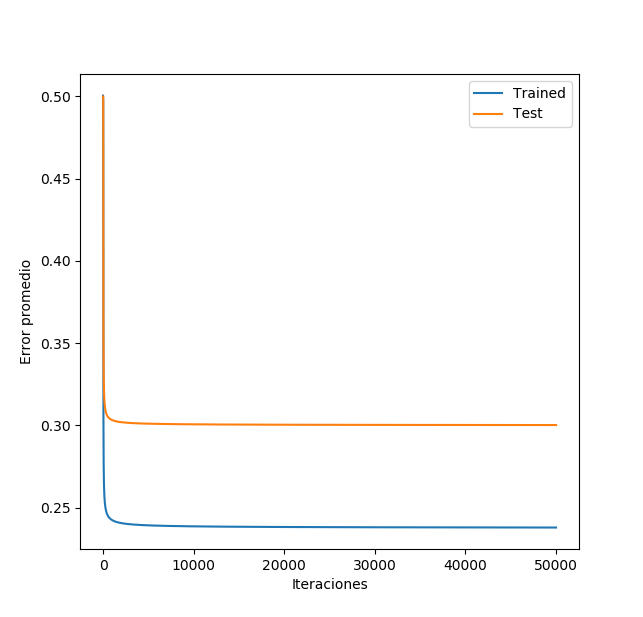
\includegraphics[width=10cm, height=8cm]{result_1hn}
    \centering
    \caption{Entrenamiento con 1 neuronas en la capa oculta}
    \label{fig:result_1hn}
\end{figure}
\subsubsection{Entrenamiento con dos neuronas en la capa oculta}
Con eta=0.08 y hasta alcanzar la \'epoca 15000 se consigui\'o un error de 0.004, en la gráfica \ref{fig:result_2hn} se puede observar como el error del grupo de prueba obtiene un error menor hasta la \'epoca 5000, despu\'es de la muestra de entrenamiento alcanza a la de prueba, obtienendo errores promedio similares.
\begin{figure}[H]
    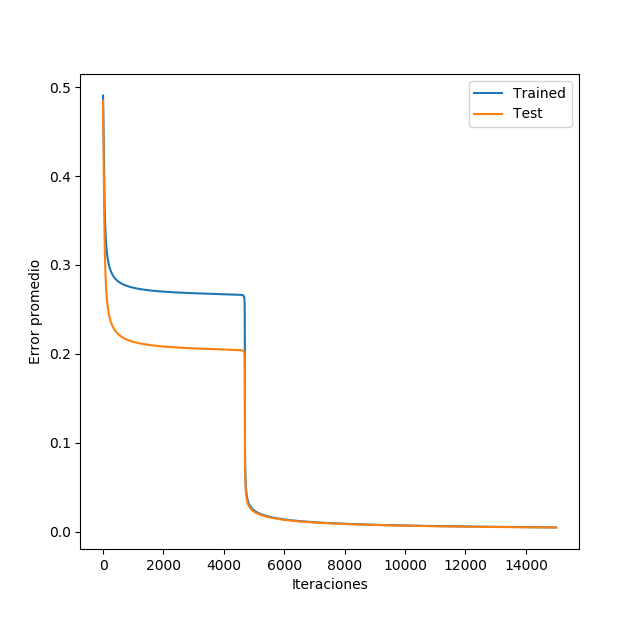
\includegraphics[width=10cm, height=8cm]{result_2hn}
    \centering
    \caption{Entrenamiento con 2 neuronas en la capa oculta}
    \label{fig:result_2hn}
\end{figure}
\subsubsection{Entrenamiento con tres neuronas en la capa oculta}
Los resultados obtenidos bajo esta arquitectura usando eta=0.35 y funci\'on de activaci\'on sigmoide
hasta alcanzar la \'epoca 15000 se observan en la figura \ref{fig:result_3hn}. Se puede observar como el error promedio con los datos de entrenamiento y de prueba
se reduce constantemente hasta alcanzar el valor de 0.001460.
\begin{figure}[H]
    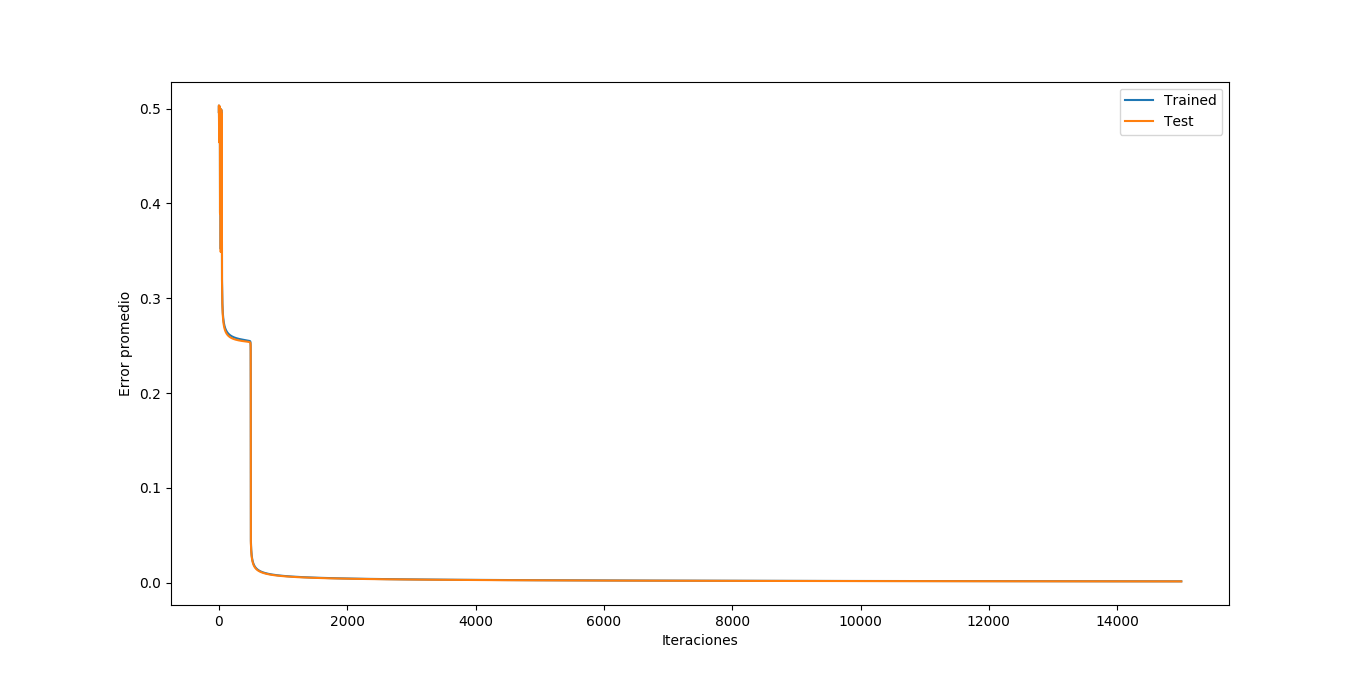
\includegraphics[width=10cm, height=8cm]{result_3hn}
    \centering
    \caption{Entrenamiento con 3 neuronas en la capa oculta}
    \label{fig:result_3hn}
\end{figure}
\end{document}
